\section{What information can eliminate}
\label{sec:information}
\subsection{Blackwell improvement for a pure information action}
\begin{proposition}[Standard information monotonicity]
\label{prop:blackwell}
Replace a pure verification channel $P$ by $\widetilde P$ on the same hidden
environment, where $P=\widetilde P G$ for an environment-independent stochastic
garbling matrix $G$. Suppose verification has the same environment-wise cost
in both models, independent of its signal, and leaves the visible state unchanged
(or makes the same deterministic budget transition); all other primitives are
unchanged. Then the unrestricted optimal
Bayes loss cannot increase, at any finite horizon or initial belief.
\end{proposition}
\begin{proof}
After each fine-channel observation, a controller can sample the garbling and
run any coarse-channel policy on the resulting fictitious coarse history. Its
joint law of environments, coarse observations, actions, states, and losses
matches that in the coarse model. The fine model admits this randomized policy,
and a deterministic optimum is no worse. Taking the infimum over coarse policies
proves the result.
\end{proof}
This is the usual experiment-comparison argument \citep{blackwell1953}.
It compares total optimal value, not a static ranking of arbitrary interventions.
Changing the representation, state transition, or verification cost violates
the comparison's assumptions. Also, a gate based on the full posterior can
change which actions are permitted after refinement, so the same simulation
argument does not automatically prove monotonicity of the gated optimum.

\subsection{An informative gate need not have a linear cost}
Augment the binary family of Proposition~\ref{prop:noinfo} with a repeatable
verification action. Each verification consumes a round, leaves the old
representation in place, incurs its old task loss plus $c_v>0$, and yields an
independent observation from $P_i$ under environment $i$. Assume a finite
alphabet, distinct full-support $P_0,P_1$, deterministic repair, and no
post-repair information. There is no fallback or deferral. Keep and repair
retain their earlier meanings and costs, including the symmetric terminal cost.
All parameters are fixed as $T$ increases.

For $0<p<1$, define
\begin{equation}
\rho=\sum_y\sqrt{P_0(y)P_1(y)}<1,\qquad \beta=-\log\rho>0.
\end{equation}
Consider the following feasible gated policy: verify exactly $n\le T-1$ times,
estimate the environment by the posterior MAP rule, repair if it estimates
$I=1$, otherwise keep, and then execute tasks to the horizon. Report the
adequacy label implied by the inferred environment and the final representation.
On a posterior tie, choose $I=1$, which is gate-feasible.

\begin{theorem}[Finite bound and logarithmic gate-cost upper bound]
\label{thm:log}
The preceding policy satisfies
\begin{equation}
J_T(\pi_n)\le
n(pr+c_v)+c_r+
\bigl[(T-n)\max(r,s)+\lambda\bigr]\sqrt{p(1-p)}e^{-\beta n}.
\label{eq:testingbound}
\end{equation}
For all sufficiently large $T$, choose
$n_T=\lceil2\log T/\beta\rceil\le T-1$. Then
\begin{equation}
0\le V_T^G(p)-V_T(p)\le J_T(\pi_{n_T})=O(\log T).
\label{eq:logbound}
\end{equation}
Consequently, a lower bound $cT-C$ with fixed $c>0$ cannot hold for this
informative family for all sufficiently large horizons.
\end{theorem}
\begin{proof}
Let $z$ be the length-$n$ verification transcript. The Bayes MAP error is
\begin{align*}
\epsilon_n&=\sum_z\min\{(1-p)P_0^n(z),\,pP_1^n(z)\}\\
&\le \sqrt{p(1-p)}\sum_z\sqrt{P_0^n(z)P_1^n(z)}
=\sqrt{p(1-p)}\rho^n,
\end{align*}
using $\min(a,b)\le\sqrt{ab}$ and independence.
The verification phase has expected cost $n(pr+c_v)$. There is at most one
repair costing $c_r$. If the MAP decision is correct, the selected
representation has zero remaining task loss; if it is wrong, the loss per
remaining round is at most $\max(r,s)$. The terminal error probability is
$\epsilon_n$, because the chosen representation's label agrees with the
declaration exactly when the environment estimate is correct. This proves
\eqref{eq:testingbound}. A repair occurs only at a posterior at least $1/2$, so
the policy is gate-feasible. With $n_T$ the exponential term is at most $T^{-2}$,
and the first term grows at most logarithmically. Finally $V_T\ge0$ and
$V_T^G\le J_T(\pi_{n_T})$ give \eqref{eq:logbound}.
\end{proof}

The theorem is an upper bound, not a matching characterization of the gate gap.
The gap may be bounded or zero in other instances. The bound also does not
extend to a fixed verification budget, unidentifiable channels, costs growing
with $T$, or repairs with nonzero residual loss in their intended environments
without further analysis.

For numerical illustration, we evaluate fixed-prefix policies exactly using
binomial counts with $p=3/10$, $P_0(Y=1)=1/5$, $P_1(Y=1)=4/5$, $r=2$,
$s=1/2$, $c_r=1$, $c_v=1/4$, and $\lambda=1$. For each plotted horizon, we
minimize over $0\le n\le\min(100,T-1)$. This is the best \emph{tested prefix},
not the unrestricted gated optimum. The environment oracle has loss $pc_r=3/10$
for the reported horizons, and
$J_T(\pi_n)-3/10$ is a valid upper bound on the gate gap.

\begin{figure}[ht]
\centering
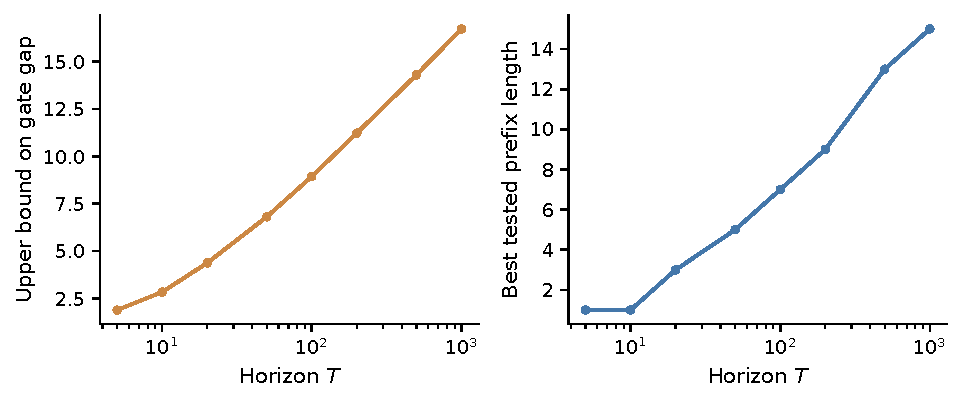
\includegraphics[width=.94\linewidth]{figures/informative_gate_bound.pdf}
\caption{A constructive upper bound when verification is repeatable and
identifiable. Left: tested fixed-prefix policy cost minus the oracle lower
bound. Right: its selected prefix length. These are not measurements of the
exact gated optimum at the large horizons.}
\label{fig:log}
\end{figure}

\subsection{Why the two boundaries coexist}
Equation~\eqref{eq:linear} concerns a controller that cannot acquire new
environment evidence. Equation~\eqref{eq:logbound} concerns one that can repeatedly
buy informative evidence. The former does not imply a universal linear
separation principle, and the latter does not remove the finite-horizon
counterexample of Theorem~\ref{thm:counter}. A short deadline, the task cost of
verification, and what repair makes observable can all influence the optimal
sequence. They must be compared under one explicit action and loss contract.
